\section{Event Reconstruction}
\label{sec:Reconstruction}

There are several software packages responsible for reconstructing tracks, showers and other objects in the near detector. Depending on the sub-detector, the base reconstruction packages are designed and optimized for different purposes. For example, the TPCs and the FGDs together form the ``Tracker", which has reconstruction optimized to separate and reconstruct tracks. The P0D on the other hand has software optimized primarily for shower reconstruction. While this is useful for analyses involving interactions with electromagnetic showers, in our case it is sub-optimal. To work around this issue, we use both reconstruction software from the P0D and the Tracker for our analysis. In addition to the base reconstruction packages, we also use algorithms to pair together reconstruction results from the separate sub-detectors.

Once we have reconstructed tracks and vertices from a series of algorithms, we apply a cut-based selection to identify candidate muon tracks. Event selection cuts are applied to exclude cosmics and other non-beam related interactions as well as to ensure that the neutrino vertex is within the water target. In this section, we first describe the individual reconstruction algorithms used by the P0D and the Tracker. Then we cover the additional reconstruction algorithms used by this analysis and finally the exact selection process for $\nu_\mu$ charged current interactions. The base tools were developed by various reconstruction groups in the T2K experiment. However, I was heavily involved in developing the analysis specific track matching algorithm in Section \ref{sec:matching} and also contributed to the momentum reconstruction algorithm in Section \ref{sec:momrecon}.

\subsection{Common Reconstruction Tools}
\label{sec:commonrecon}

The tools used by the Tracker and P0D reconstruction packages are the same in some cases. The primary external toolkit used for standardized fitting algorithms, propagation of reconstructed objects through spacetime and matching of prior reconstruction objects are performed by a package called RecPack \cite{recontn}. 

In RecPack, a Kalman filter is the main technique used for fitting geometric objects to individual detector measurements such as scintillator hits. Following a generalized Kalman filtering procedure, the algorithm takes a seed state and iterates over each measurement to adjust the seed state. The end result is a seed state that has been adjusted according to all the available detector measurements. This can be a track or shower depending on the original seed state used to start the Kalman filter iterations. The Kalman filter is not only used to construct reconstruction objects from hits, but also to combine multiple reconstruction objects over adjoining sub-detectors such as the TPCs and FGDs. In this case, one of the reconstructed tracks is used as the seed and the other as the correcting measurement.

There are some notable particulars to the global use of the Kalman filter. The TPC reconstruction algorithms do not use a Kalman filter. Instead they have a custom reconstruction scheme described in the following section. However, once there is a fitted result from the TPC reconstruction algorithm, the Kalman filter uses it as a seed state to stitch it together with results from other sub-detector reconstructions. Also, in the case of the P0D, showering events are reconstructed by a similarly proprietary algorithm. The results of the shower reconstruction are also passed to the Kalman filter as a single seed state. This analysis is unconcerned with the shower fits in the P0D since muon-like tracks are the primary focus of the selection. 

\begin{figure}
\centering
\includegraphics[width=6.5in]{Figures/Reconstruction/nd280geom.PNG}
\caption{The simplified ND280 geometry used by RecPack. The YZ projection is shown where the positive Z direction corresponds roughly to the beam direction (disregarding the off-axis nature of the beam). All axis units are in mm.} 
\label{fig:nd280geom}
\end{figure}

The RecPack software also contains a simplified ND280 detector geometry. Figure \ref{fig:nd280geom} shows the YZ projection of the simplified ND280 detector geometry. The positive Z direction corresponds to the beam direction when the off-axis nature of the beam is ignored. All coordinate values used in this analysis are given with respect to this ND280 coordinate system. Material properties encoded in RecPack and used in fitting and propagation of tracks are also simplified to the bare necessities. Specifically, the radiation length and the average energy loss per unit length are stored. The average energy loss is calculated using the proper Bethe-Bloch equation curves for each material. 

\subsection{TPC Reconstruction}
\label{sec:tpcrecon}

The three Time Projection Chambers in ND280 use custom reconstruction software to reconstruct tracks from collections of Micromega hits. Each TPC reconstructs objects separately. The details of full track stitching over the entire Tracker segment of ND280 is described in the Tracker reconstruction section.

\begin{figure}
\centering
\includegraphics[width=5.5in]{Figures/Reconstruction/tpcrecoflow.PNG}
\caption{A flow chart showing the steps in the TPC reconstruction algorithm used by each chamber separately. The steps are described in the text.} 
\label{fig:tpcrecoflow}
\end{figure}

Figure \ref{fig:tpcrecoflow} shows a flow chart summarizing the many steps of the TPC track reconstruction procedure. To reconstruct TPC tracks, Micromega hits are first passed through a calbration process. Gain constants are applied and dead/noisy channels are removed from the list of good Micromega hits. Once a collection of above noise hits are identified, the algorithm searches for clusters along each Micromega column. Discovered clusters are joined together to form tracks using pattern recognition software based on a cellular automaton algorithm. The general steps in the algorithm are as follows:

\begin{enumerate}
\item Clusters in contiguous Micromega columns are connected. These sets of connected clusters are called segments.
\item Connect segments together if they overlap in time and space.
\item Stepwise algorithm selects the list of connected segments that form the longest physical track. The algorithm is allowed to skip a predefined number of unfired Micromega columns. This number is optimized by TPC reconstruction experts.
\item Likelihood fit is used to fit a helix to the resulting sequence of hits.
\end{enumerate}

As Micromega columns are only placed along the Y-axis of the TPCs, only the YZ projection has any reconstructed tracks at this point. Once a YZ track object is fitted by the pattern recognition algorithm, the next step identifies the $t_0$ of the track in order to reconstruct the XZ direction as well. As is common with time projection chambers, the $t_0$ value in conjunction with the known drift velocity in the TPC gas and the relative ion arrival times allows track reconstruction along the drift axis. To find the $t_0$, the YZ track is first extrapolated to adjacent sub-detectors by RecPack. If there are hits in the adjacent sub-detectors, the algorithm searches for the hit-track pair with the lowest YZ plane residual. Hits in FGDs are given first priority for matching, followed by the barrel ECAL and then the P0D. As the adjacent sub-detectors are all scintillator based, the matched hit provides a time stamp. This time stamp is then used as the $t_0$ value after cross detector timing corrections. In the case that no hits are available in the adjacent sub-detectors and the TPC track crossed the cathode plane, the time stamp from the cathode plane measurement is used as the $t_0$. Given the long, multi-detector nature of tracks selected in our analysis, this particular $t_0$ determination mode is not of often used.

\subsection{FGD Reconstruction}
\label{sec:fgdrecon}

After the TPC reconstruction algorithm is complete, the FGD reconstruction software takes over. There are a few major steps in the FGD reconstruction process. They are:

\begin{enumerate}
\item FGD hits are separated according to hit time stamps;
\item TPC tracks are matched to FGD hits;
\item Collect hits unmatched to TPC tracks and reconstruct them into FGD-only objects.
\end{enumerate}

The first step in the algorithm clusters FGD hits together into time bins. Beginning with a single hit, others are collected into the same time bin as long as the time difference between consecutive hits is below a predetermined cut value. When the time difference between hits is too large, a new time bin is created and the clustering process is repeated. Once all hits are clustered in time, algorithm runs over each time bin individually.

In the second step, the previously reconstructed TPC tracks are matched and then stitched together with FGD tracks. RecPack first  extrapolates each TPC track to the closest FGD layer. A chi-squared value is calculated between the extrapolated point and the FGD hit. If the chi-squared value is below a preset cut value, the FGD hit is considered matched with the seed TPC track. Following the Kalman filtering procedure, the original, TPC-only track seed state is recalculated using the matched FGD hit. The seed is then extrapolated to the next closest FGD layer and the process is repeated until all the hits are collected into the track state. The end result is a TPC track combined with all the hits in an adjacent FGD to form a two-detector track fit. Tracks from each TPC are matched with hits from the adjacent FGDs. Specifically, TPC1 is matched with FGD1, TPC2 is matched with FGD1 and FGD2, and TPC3 is matched with FGD3. In the case of TPC2, there are two combinations of reconstructed tracks: the TPC2-FGD1 combination and the TPC2-FGD2 combination. Finally, these results are passed to the Tracker reconstruction algorithm. We do not cover the FGD-only reconstruction algorithm as it is not used by any tracks selected in our analysis.

\subsection{Tracker Reconstruction}
\label{sec:trackerrecon}

The Tracker reconstruction algorithm is responsible for stitching together the results from the chain of TPC and FGD reconstruction algorithms. As this package only works with already fitted objects, it comprises a simpler set of steps than the sub-detector packages. First, the Tracker reconstruction uses RecPack to stitch together multi-TPC tracks into longer objects. All the TPC-FGD track pairs created in the previous step are iterated over searching for overlaps. All sets of TPC-FGD tracks that have a chi-squared per number of degrees of freedom (NDOF) of less than 100 are considered a match and stitched together by RecPack. Using the Kalman filter, these sets are fit together into one cohesive multi-TPC, multi-FGD track object. The process is repeated with any remaining TPC-FGD pairs. In the final step, the algorithm determines the directionality of the entire track. For multi-FGD tracks, a track with an FGD2 time stamp 3~ns before its FGD1 time stamp is determined to be a ``backwards'' going track. Such tracks are traveling anti-parallel to the the neutrino beam and are often a result of a background cosmic track occurring in a beam event. The proper reconstruction of track direction is also crucial in determining the sign of the particle. Any uncertainty here translates into a small uncertainty in the number of selected negative muon tracks, the primary target for our selection. This error is evaluated later as a systematic uncertainty.

\subsection{P0D Reconstruction}
\label{sec:p0drecon}

The P0D reconstruction package runs independently of and parallel to the entire Tracker reconstruction algorithm chain. There are two major sections in the procedure, one for track reconstruction and another for shower reconstruction. Figure \ref{fig:p0drecoflow} shows a flow chart that breaks down the modular P0D reconstruction algorithm we use. We ignore all shower objects in the P0D as they are of no interest in our selection. Therefore, in this section we will only cover the details of track reconstruction in the P0D. 

\begin{figure}
\centering
\includegraphics[width=6in]{Figures/Reconstruction/p0drecoflow.PNG}
\caption{A flow chart showing the steps in the P0D reconstruction algorithm used to create both track and shower objects. The steps are described in the text.} 
\label{fig:p0drecoflow}
\end{figure}

The P0D electronics are designed to have 23 separate charge integration windows separated by a 100~ns. For each beam trigger, the electronics cycle through 23 integration windows where the 6-8 beam spills fall squarely into a known set of 6-8 of integration windows. The number of beam spills depends on the beam run number. The first beam run had exactly 6 beam spills per trigger and all others had 8 beam spills per trigger. As events from each beam spill are presumed to be independent, the reconstruction algorithm runs separately on each integration window. 

The first step of P0D reconstruction involves the removal of noisy hits and the construction of track seeds. To be considered signal, each hit must pass at least one of the following noise cuts:

\begin{itemize}
\item Calibrated charge deposited in the scintillator bar (Q) is greater than 15 photoelectron equivalent units (peu) .
\item The hit Q is greater than 7~peu and there is an adjacent hit within 30~ns of it within a 10~cm radius
\item The hit has a neighboring hit within 30~ns and 3.5~cm. This distance is on the order of a single P0D scintillator bar. No Q cut is applied.
\end{itemize}

Any integration window with fewer than 5 signal hits is ignored. The remaining list of hits is referred to as ``cleaned'' hits. This list is first passed to the tracking algorithm. To collect hits into the desired tracks, the XZ and YZ projections are first considered independently. Track seeds are constructed by using a Hough transform with bin sizes of 1.8$\degree$ and 25~mm. A Hough transform is a common image processing tool used in this case to find simple lines in the XY and YZ projections. First, a line is parametrized as $r = x \cos\theta + y \sin\theta$. Then for every hit, a function relating $r$ and $\theta$ is plotted by calculating the orthogonal distance from the origin to a line passing through the hit with angle $\theta$. This process is repeated for all the hits. If there is a line that passes through multiple hits, this manifests as multiple $r-\theta$ functions intersecting at a single point. The intersection point yields the best fit line. Only seeds with at least 4 hits are considered. These seeds are then extended with a road following algorithm that adds hits to the seed. The ``road'' is allowed to be 60~mm wide and within 1.5~rad of the seed direction. If a P0D layer has a hit that would be included by the road following algorithm, then up to 3 adjacent hits in the same layer are also added to the track seed. Once the road following algorithm reaches the last layer with hits, up to 4 extra hits at either end of the track are non-exclusively added to the track seed. In the likely case that there are multiple tracks originating from an event vertex, this allows multiple tracks to share the same vertex position. Finally, resulant track seeds are merged together if they satisfy two requirements. First, the beginning of a downstream track must be within 100~mm of the end of an upstream track. This distance is on the order of the thickness of 1 P0Dule. And second, half of the nodes of the downstream track is within a 0.2~rad cone of direction of the upstream track's tail-end. 

Once the algorithm constructs XZ and YZ tracks in all possible cycles using the described procedure, the two views are matched together to create 3D P0D tracks. Each 2D track is compared to all 2D tracks in the other view and a matching score is calculated. This score depends on the number of overlapping layers and the disparity between the total deposited charge of each track pair as well as whether the tracks have already been matched elsewhere. The pairings with the best score are selected as proper XZ-YZ track matches. The 3D track is then reconstructed by the RecPack Kalman filter using the collected hits as measurements. Once the Kalman filter provides a geometric track object, the intersection of the track and each P0D layer is stored as a P0D Node object. These P0D Node objects are extremely useful for selection cuts as well as studies of detector systematic uncertainty. They are used in several areas in this analysis. In the case of some very short or steep tracks with few hits, a Kalman filter procedure would not provide a meaningful or robust result. For these tracks, a parametric fitting method is used by simply fitting a line to the hits. The number of tracks using this fitting method is fractionally negligible in our selection.

The shower reconstruction algorithm collects the appropriate fitted tracks into showers. And finally a simple vertexing algorithm uses multiple tracks and showers to create a prediction for the vertex location. These two pieces of the reconstruction algorithm, though important for showering analyses, are not relevant in our case and therefore not discussed. Our selection only examines long tracks in the P0D and entirely ignores showers. Also, MC studies suggest that in the case of single, long muon-like tracks, the position of the most upstream P0D Node of the track is actually a more accurate predicition of the event vertex. The uncertainties inherited from such an assumption are treated appropriately in a later section on detector systematics.

\subsection{Track Matching Algorithm}
\label{sec:matching}

 The individual track reconstruction results from the P0D and the Tracker software are combined together to form longer, inter-detector tracks. We use a relatively straightforward method to pair together tracks from the P0D and the Tracker that avoids any double counting as well as yields acceptable rate of successful matches. 

Each P0D and Tracker track is checked for quality and to make sure that they are likely multi-detector tracks. The quality check ensures that the individual reconstruction packages succeeded. The multi-detector check allows us to eventually find muon candidate tracks that have reconstructible momentum and resolvable interaction vertex position and track direction. For example, a track originating in the P0D and also ending in the P0D would have resolvable vertex position and track direction, but no measurable momentum from the TPC. 

The quality checks are as follows:
\begin{itemize}
\item The P0D Track is 3D. This is defined by examining the variance of the fitted vertex position. We only require that the variance of vertex position not be impossibly large. Specifically, we make cuts of X, Y and Z vertex position variance, requiring that they are less than $10^8$~mm (an uphysically large default failure value). This assures us that the fitting algorithm succesfully reconstructed both the XY and YZ projections of the track and properly matched them together.
\item The Tracker Track has greater than 18 nodes. Studies done on the reconstruction power of the Tracker algorithms suggest that a minimum of 18 nodes is necessary in the TPCs to find a believable particle track. This corresponds to the pixel width of 1 column of Micromegas in a single TPC. There are 4 such columns reading out each TPC.
\end{itemize}

The multi-detector checks are as follows:
\begin{itemize}
\item The P0D Track is required to exit the P0D via the downstream face. Geometrically, this is equivalent to the most downstream P0D node having a Z position $>$ -1016~mm.
\item The Tracker track is required to enter from the upstream face of the first TPC. Geometrically, this is equivalent to the most upstream position of the Tracker track having a Z position $<$ -750~mm.
\end{itemize}

The list of P0D and Tracker tracks remaining after these checks are paired together uniquely. A parameter, $\Delta$R, is calculated by measuring the distance between the backwards projected Tracker track and the end of the P0D track. Track pairs reconstructed within 100~ns of each other and with the lowest matching $\Delta$R are assigned to each other. A graphic showing how $\Delta R$ and sin($\Delta \theta$) are calculated is shown in Figure \ref{fig:dRCalc}. To avoid non-physical matches, we also require that no pairs are matched with $\Delta$R $>$ 76mm. Also, no track pairs that have a difference in polar angle greater than sin$\Delta\theta$ = 0.88 is allowed.

\begin{figure}
\begin{center}
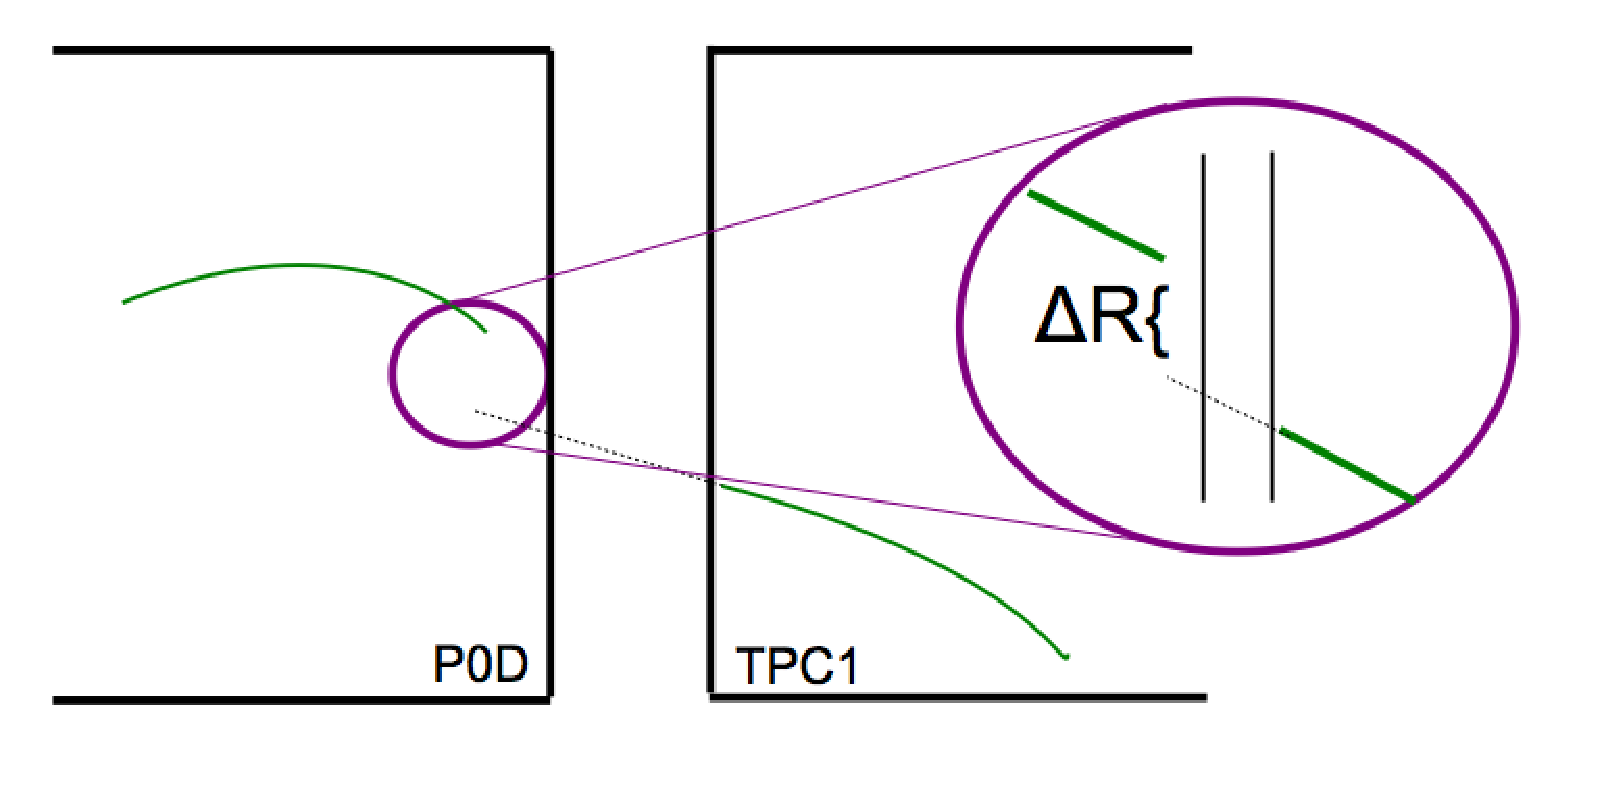
\includegraphics[width=3.2in]{Figures/drCalc.eps}
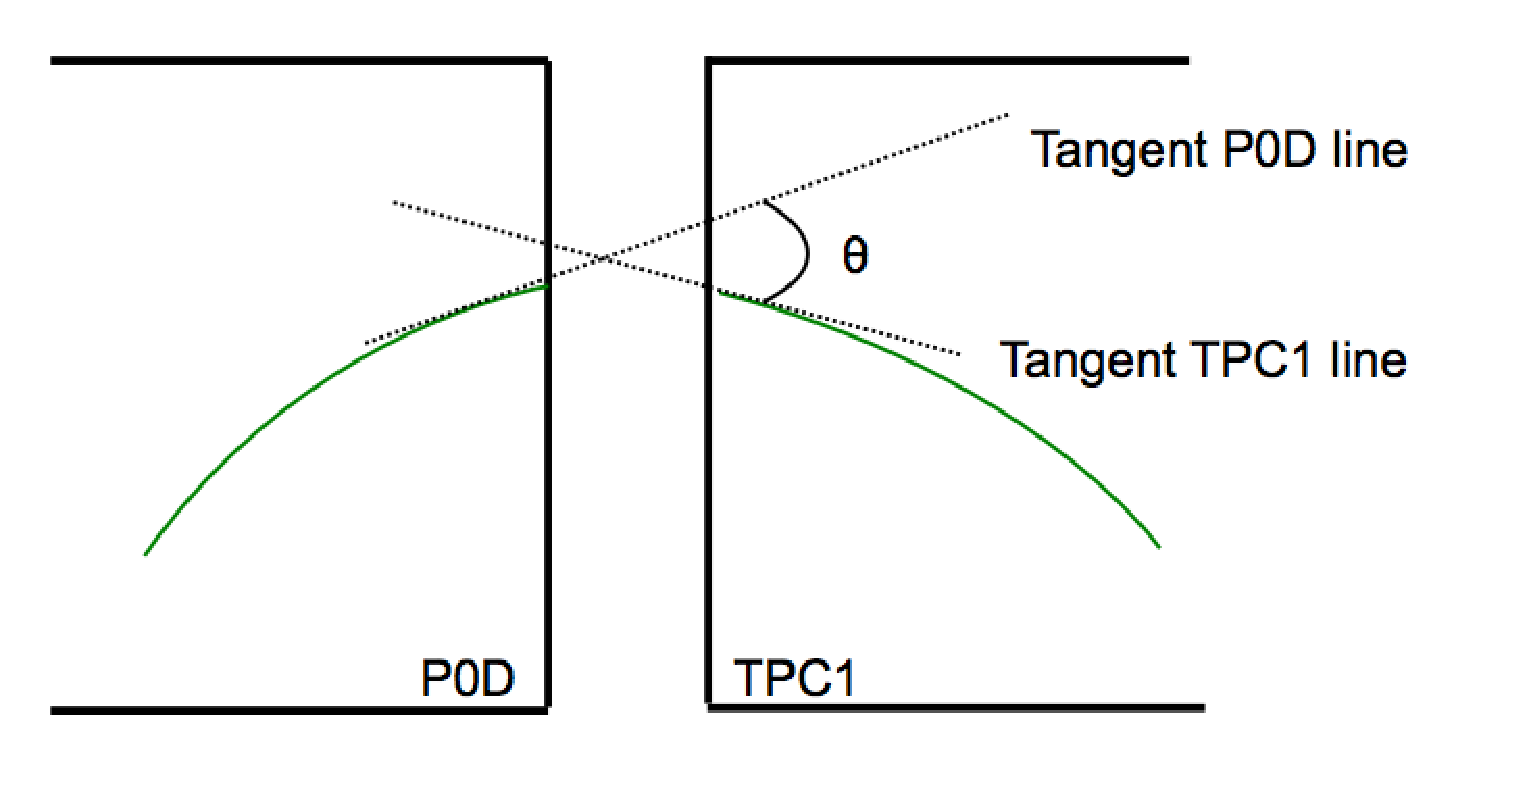
\includegraphics[width=3.2in]{Figures/sindThetaCalc.eps}
\end{center}
\caption{Graphic demonstrating how the analysis calculates $\Delta R$ (left) and sin($\Delta \theta$) (right) for the track matching algorithm.}
\label{fig:dRCalc}
\end{figure}

We use a simple figure of merit (FOM) optimization process on beam MC to determine the cut values of $\Delta$R and sin$\Delta\theta$. The chosen FOM is 
\begin{equation}
F = \frac{\delta S}{S} = \frac{\sqrt{S+2B}}{S}
\end{equation}
\noindent where S is the total number of signal events passing a certain ($\Delta$R, sin$\Delta\theta$) cut, B is the background and $\delta S$ is the error. The second form of the FOM comes from assuming poissonian errors on the total number of events and the number of background events B. Minimizing this figure of merit will maximize the total signal while minimizing the error on the signal. We use beam MC and follow the matching procedure described above up to the  ($\Delta$R, sin$\Delta\theta$) cut. For every pair of  ($\Delta$R, sin$\Delta\theta$) cut values, the signal is defined as the number of successfully matched tracks that have both track segments originating from the same primary true trajectory (a primary trajectory is a true particle vector leaving the original vertex). Then the background is the remainder of the tracks that were matched but were not from the same primary trajectory. A 3D FOM histogram is created (see Figures \ref{fig:FOM1} and \ref{fig:FOM2}) where each bin (i,j) is filled with the calculated FOM from the matching algorithm with cuts $\Delta$R$\leq$i and sin$\Delta\theta\leq$j. 

\begin{figure}
\begin{center}
\includegraphics[width=6in]{Figures/FOM1.png}
\end{center}
\caption{The figure of merit value as a function of $\Delta$R and sin$\Delta\theta$ cut values using run 2 water-in MC. The left side shows the entire allowed cut region and the right side is zoomed in to the local maximum (76~mm, 0.88) with the Z axis zero suppressed.}
\label{fig:FOM1}
\end{figure}

\begin{figure}
\begin{center}
\includegraphics[width=6in]{Figures/FOM2.png}
\end{center}
\caption{The figure of merit value as a function of $\Delta$R and sin$\Delta\theta$ cut values using run 3 water-out MC. The left side shows the entire allowed cut region and the right side is zoomed in to the local maximum (78~mm, 0.90) with the Z axis zero suppressed.}
\label{fig:FOM2}
\end{figure}

The FOM does not vary wildly over the scanned cut values. In fact, we have to zoom into the optimal region to even see where the local maxima is located. These maxima are shown in the right hand histogram in Figures \ref{fig:FOM1} and \ref{fig:FOM2}. They are at the coordinates (76~mm, 0.88) and (78~mm, 0.90) for water-in and water-out samples respectively. To simplify the selection procedure, we use the more stringent of the two cut choices, specifically $\Delta$R $\leq$ 76~mm and sin$\Delta\theta\leq0.88$ for all data and MC samples. Finally, we also investigate the agreement between data and MC in the distributions of the matching parameters. Large differences in the $\Delta$R and sin$\Delta\theta$ distributions of data and MC would cause a systematic difference in our data and MC selection efficiencies. This effect is accounted for by detailed systematic studies on the matching efficiency conducted in Section \ref{sec:matchingsyst}, but we also show in Figures \ref{fig:matchpar1} and \ref{fig:matchpar2} that the pre-cut data and MC distributions of $\Delta$R and sin$\Delta\theta$ track each other quite well near the cut values. Note that as the MC we use does not simulate external interactions, we apply a loose vertex position cut ($Z>$ -3183~mm, $|X|$ and $|Y|<$ 1000~mm) on the data.

\begin{figure}
\begin{center}[h]
\includegraphics[width=6in]{Figures/matchpar1.png}
\end{center}
\caption{The pre-cut $\Delta$R (left) and sin$\Delta\theta$ (right) distributions for data (black) and MC (red) using run 2 water-in samples.}
\label{fig:matchpar1}
\end{figure}

\begin{figure}[h]
\begin{center}
\includegraphics[width=6in]{Figures/matchpar2.png}
\end{center}
\caption{The pre-cut $\Delta$R (left) and sin$\Delta\theta$ (right) distributions for data (black) and MC (red) using run 3 water-out samples.}
\label{fig:matchpar2}
\end{figure}

\subsection{Track Momentum Reconstruction}
\label{sec:momrecon}

To reconstruct the momentum of the muon track, we use the momentum measurement from TPC1 made by fitting a helix to the track and comparing the curvature to the local magnetic field. This momentum is then corrected for the segment of the track that passed through the P0D. Using muon range tables in conjunction with the known materials density in the different P0D regions, we can calculate the momentum of the muon at the vertex by adding in the total energy lost. As we must do this for every single muon-like negative track in every event, we require that the algorithm is fast. So we chose not to use $\frac{dE}{dx}$ tables to incrementally restore the energy lost. Instead, the P0D energy loss was calculated using range data for the two types of superP0Dules: water target and ECAL. Range is defined as
\begin{equation}
R(E') = \int^{E'}_{0} \left(\frac{dE}{dx}\right)^{-1} dE
\end{equation}
where $\frac{dE}{dx}$ is the weighted average energy loss over all materials. The range is calculated for each superP0Dule. This gives us a table of range vs energy/momentum for each section of the P0D and avoids performing the integration every single time a track is found. The track length in the P0D is used to find the corresponding energy lost (see Figure \ref{fig:eloss}) and add it to the TPC1 measurement momentum. If the track traversed through mutiple superP0Dules, as it must, then the energy loss look-up procedure is performed separately for each. The momentum residual as defined by $(P_{reco}-P_{truth})/P_{truth}$ for run 2 water-in and run 3 water-out samples is shown in Figure \ref{fig:momres} for reference. The algorithm does an excellent, unbiased job of reconstructing muon momenta according to MC.

\begin{figure}
\centering
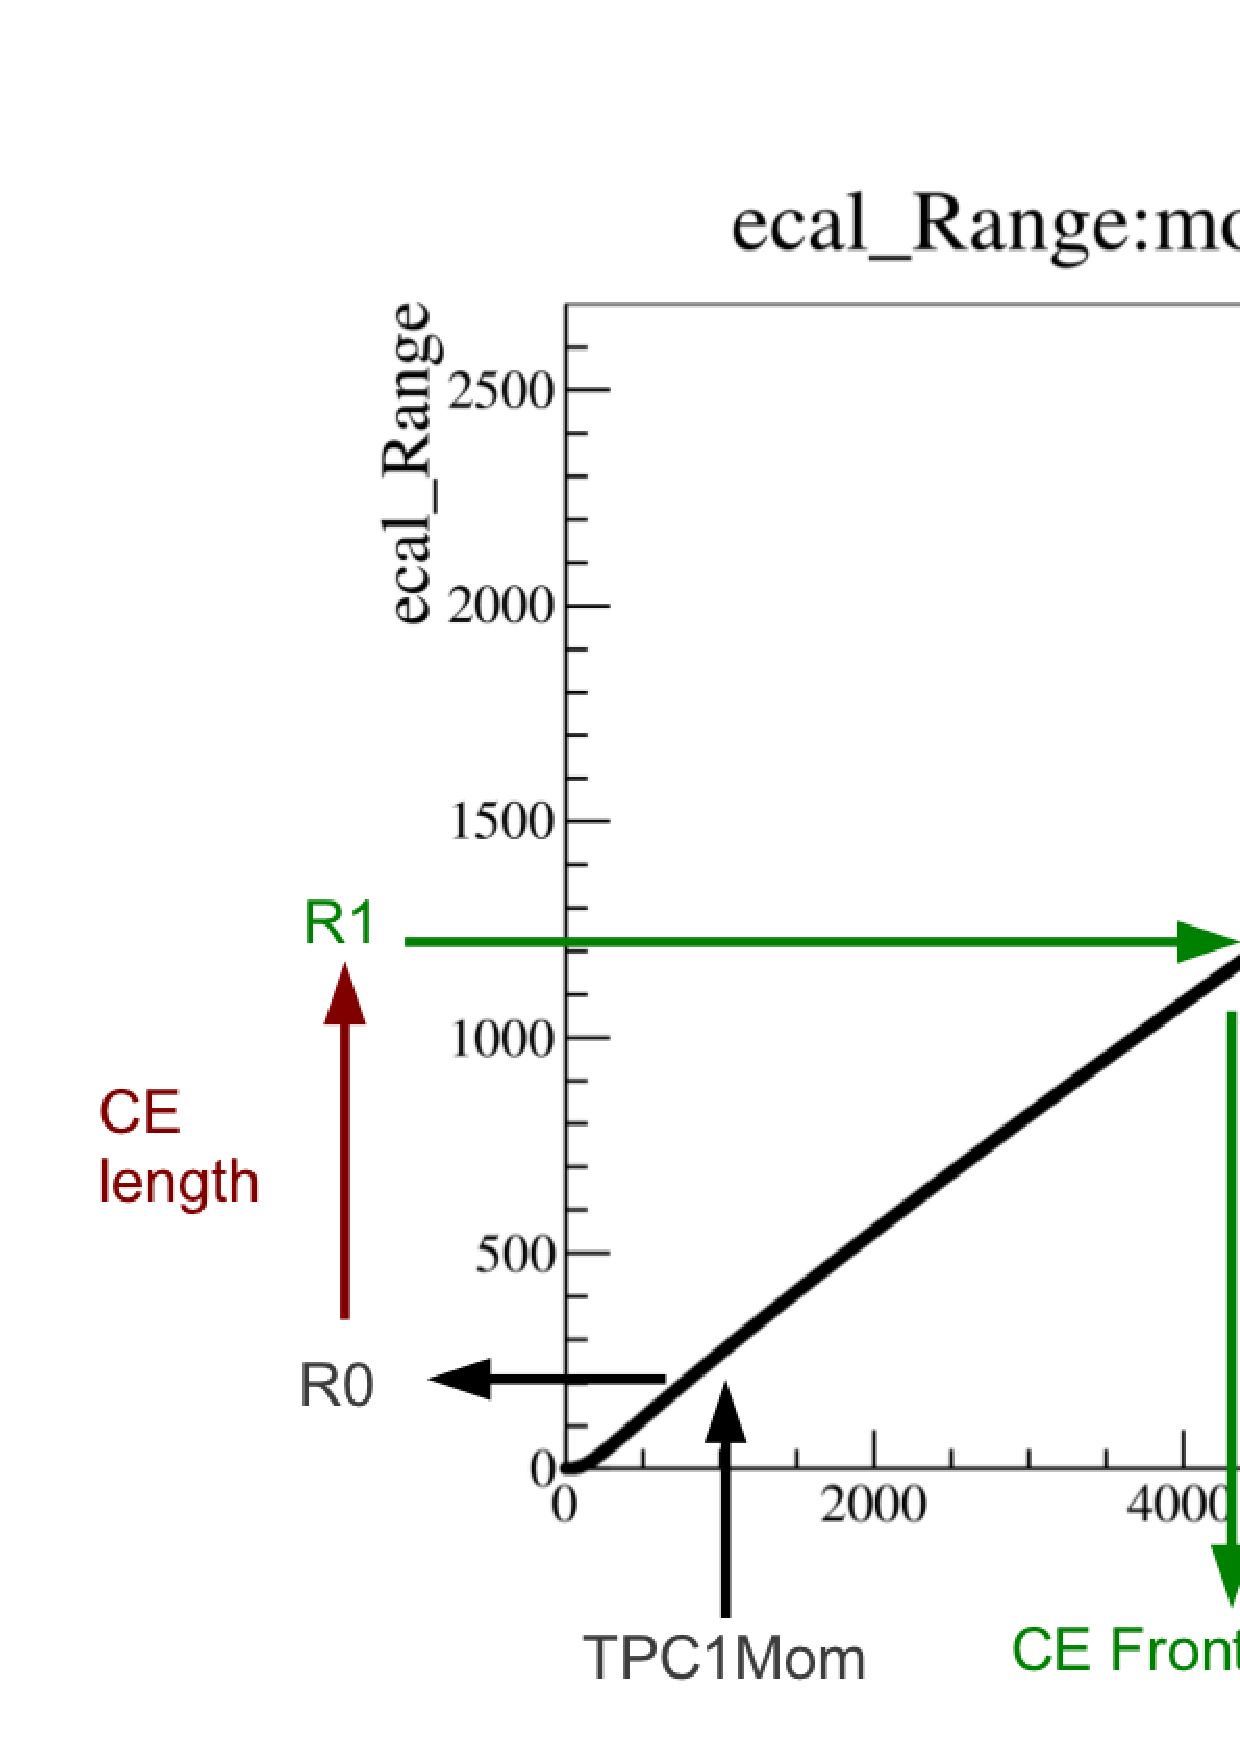
\includegraphics[width=5.5in]{Figures/eLossCalc1.png}
\caption{Calculation of P0D momentum correction. The steps of the correction
are shown schematically with the arrows} 
\label{fig:eloss}
\end{figure}

\begin{figure}
\centering
\includegraphics[width=5.5in]{Figures/momentumresidual.png}
\caption{The momentum residual comparing the reconstructed momentum with the true track momentum in run 2 water-in MC (blue) and run 3 water-out MC (purple).}
\label{fig:momres}
\end{figure}
